% \chapter{Многоспиновая запутанность в зигзагообразной цепочке}
\chapter{Многоспиновая запутанность в квазиодномерных цепочках}
\label{chapter:manayparticle-entantlement-in-zigzag-chain}
% AMR-2020


% \begin{figure}
%   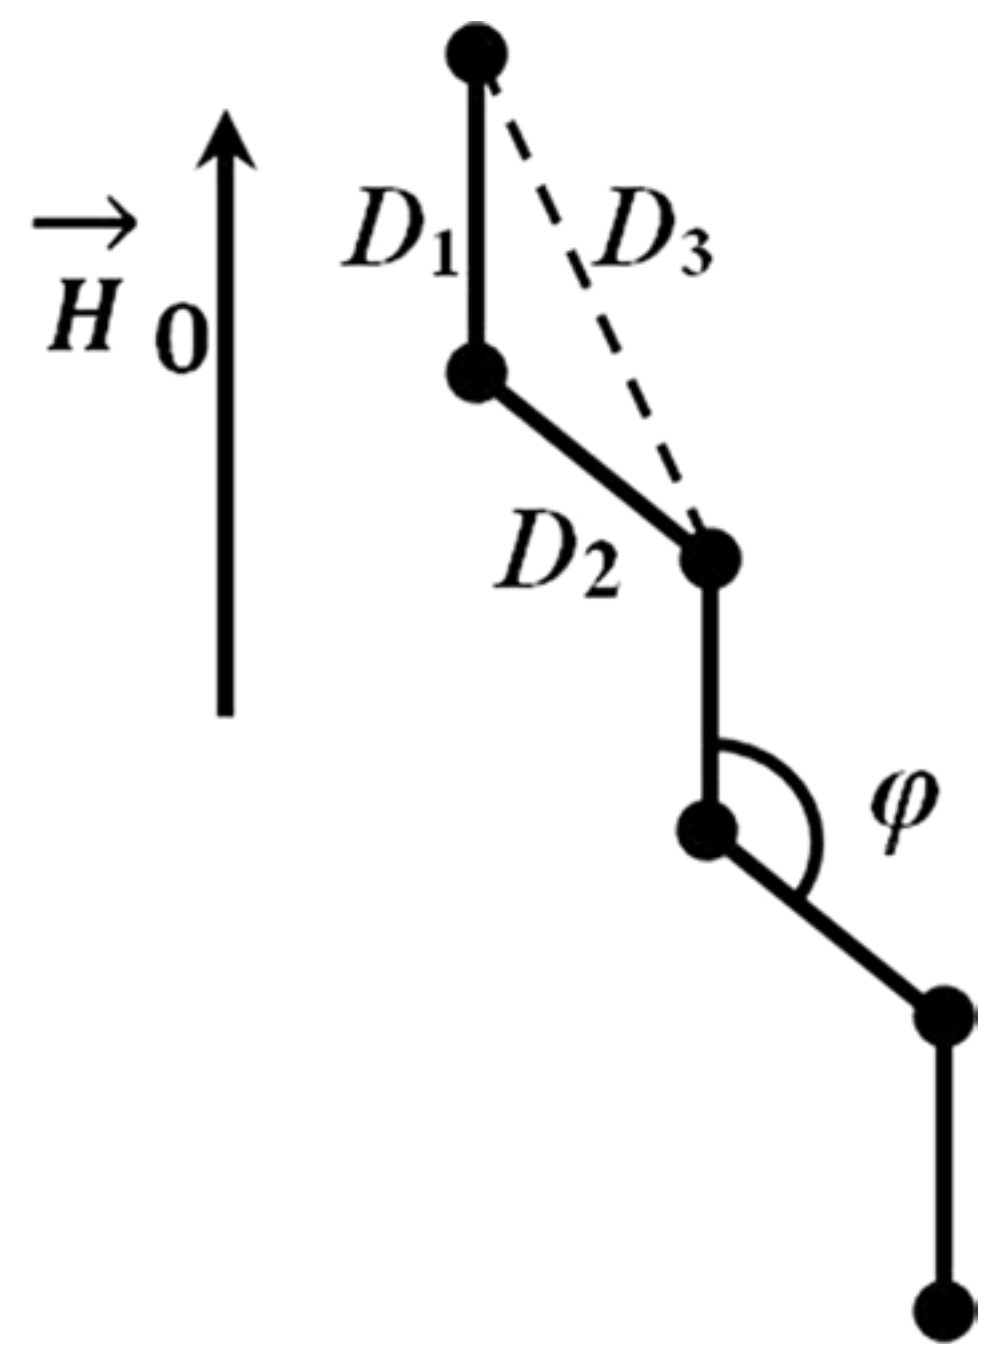
\includegraphics[width=0.5\textwidth]{model-zigzag-chain-schema.png}
%   \caption{Схема зигзагообзаной цепочки}
% \end{figure}
%
%     Константы взаимодействия
%         $$D_1=\dfrac{\gamma^2\hbar }{r^3}, $$
%         $$D_2 = D_1\dfrac{ 3\cos^2 \varphi -1 }{2} $$
%         $$D_3 = D_1 \dfrac{ 3\sin^2 \frac{\varphi}{2} -1}{16 \sin^3, \frac{\varphi}{2}}$$
%         где $\gamma$ - гиромагнитное отношение,
%         $\varphi$ - угол между соседними связями,
%         $r$ - расстояние между соседними спинами в цепочке.
%
%     Базовый случай это когда одна линия связи направлена вдоль поля. тогда констаты будет самой большой в доль поля.
%     Изменяя угол к полю мы можем получить как альтернированную цепочку так и однородную.
%     В приближении ближайших и следующих соседей, задача решается аналитически, но она
%     не дает полной картины. Поэтому мы решали данную систему численно.
%
%     \begin{figure}
%       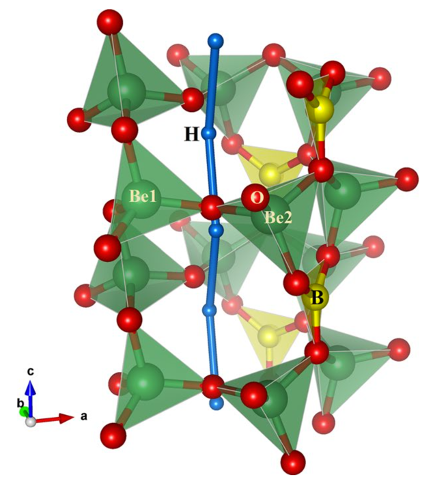
\includegraphics[width=0.85\textwidth]{model-zigzag-chain-hambergite-structure.png}
%       \caption{Hанопора со спин-несущих молекулами во внешнем сильном магнитном поле $\vec B$}
%     \end{figure}
%
%     Гамбергит $Be_2BO_3(OH)$
%         \begin{itemize}
%             \item Дипольное взаимодействия между ближайшими спинами протонов в цепи в 17 раз сильнее, чем со спинами окружающих цепей (в худшем случае).
%             \item Взаимодействия с остальными окружающими спинами по меньшей мере в 30 раз слабее.
%             \item Вклад дипольной связи между спинами в одной и той же цепи доминирует над остальными взаимодействиями.
%         \end{itemize}
%
%     В одномерных цепочках возникают когерентности только $\pm 2$ порядка
%     и следовательно дисперсия распределения будет небольшой
%     и мы не увидим запутанных кластеров.
%     Однако в альтернированная цепочке гамбергита возникают когерентности $\pm 4$ порядка
%     и следовательно можно использовать эту модель для исследования многочастичной запутанности.
%     The distance to these two protons is 4.49~\r{A}
%     The distance between a given chain and surrounding proton chains is at least 2.1 times larger than the distance between neighbors in the chain.
%

В предыдущей главе~\ref{chapter:manyparticle-entanglement-in-nanopore}
была подробно исследована многочастичная запутанность,
возникающая в МК эксперименте ЯМР в нанопоре,
и эта модель показала себя отличной площадкой
для исследования взаимодействия многих частиц.
Тем не менее одномерные модели~(см. раздел~\ref{sec:model-uniform-chain})
гораздо лучше изучены как теоретически,
так и экспериментально.
В частности в таких моделях изучены процессы
декогеренции~\cite{Bochkin2018},
передачи квантовых состояний~\cite{Lazarev2019, Feldman2020, Bochkin2022},
а также возникновения бинарной запутанности~\cite{Feldman2012, Lazarev2019}.
Ввиду такого широкого представления одномерных систем в литературе,
несомненно важно рассмотреть эти системы в контексте возникновения многочастичной запутанности.

% \section{Однородная цепочка}
% \subsection{Передача квантового состояния}
% \subsection{Температурная зависимость бинарной запутанности}

\section{Зигзагообразная цепочка}
В зигзагообразных цепочках в кристалле гамбергита в МК эксперименте ЯМР возникают когерентности плюс/минус четвертого порядка (см. раздел~\ref{sec:model-zigzag-chain}).
Данное обстоятельство является важным для исследования многоспиновой запутанности,
поскольку при этом используется второй момент распределения МК когерентностей ЯМР.

\begin{figure}[H]
    \centering
    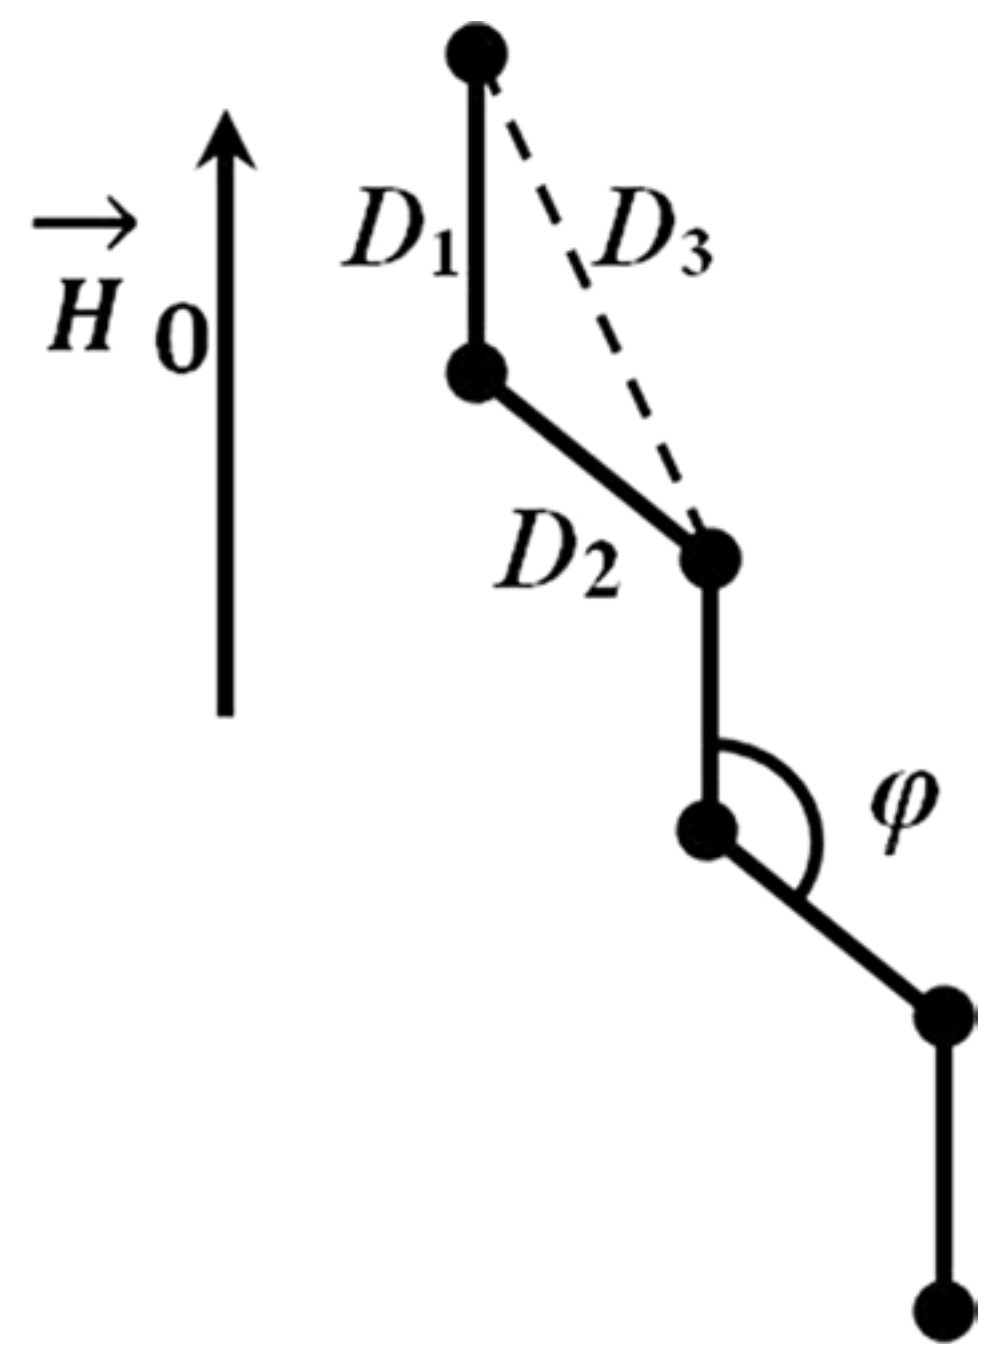
\includegraphics[width=0.3\textwidth]{model-zigzag-chain-schema}
    \caption{
      Зигзагообразная цепочка ядерных спинов.
      Нечетные звенья параллельны внешнему магнитному полю $\vec{\mathcal H}_0$,
      а $\varphi$ - угол между соседними звеньями.
      Константы связи $D_1$ и $D_2$ определяются уравнением~(\ref{eq:dipolaconstantsnearest}), а $D_3=D_{n, n+2},\, (n=1,2,...)$
      уравнением~(\ref{eq:dipolaconstantsnextnearest}).
    }
    \label{fig:model-zigzag-chain-schema}
\end{figure}

На рис.~\ref{fig:model-zigzag-chain-schema} схематично представлена
зигзагообразная цепочка ядерных спинов в сильном внешнем магнитным полем $\vec{\mathcal H}_0$.
Нечетные звенья цепочки параллельны внешнему магнитному полю $\vec{\mathcal H}_0$,
а $\varphi$ - угол между соседними звеньями.
Гамильтониан $H_\mathrm{MQ}$,
описывающий МК динамику ЯМР~(см. раздел~\ref{sec:mq-nrm-experiment}),
задается выражением~\cite{Doronin2000}
%
\begin{equation}\label{hmqnextnearest}
 H_\mathrm{MQ} = \sum_{i=1}^{N-1} D_{i, i+1}(I_i^{+}I_{i+1}^{+}+ I_i^{-}I_{i+1}^{-} )
   + \sum_{i=1}^{N-2} D_{i, i+2}(I_i^{+}I_{i+2}^{+}+ I_i^{-}I_{i+2}^{-} ) ,
\end{equation}
%
где $I_i^+$, $I_i^-$ --- это повышающей и понижающий операторы спинового углового момента спина с номером $i$,
и $N$ --- это количество ядерных спинов в цепочке.

Константы диполь-дипольного взаимодействия (ДДВ)
в зигзагообразной цепочке определяются выражениями~\cite{Abragam1982}
%
\begin{equation}\label{eq:dipolaconstantsnearest}
  D_{2n-1, 2n} = D_1 =\dfrac{\gamma^2\hbar }{r^3},
  \quad
  D_{2n, 2n+1} = D_2=\dfrac{\gamma^2\hbar }{2r^3}\p{3\cos^2 \varphi -1},
  \quad
  n=1,2\dots,
\end{equation}
где $\gamma$ --- это гиромагнитное отношение,
и $r$ --- это расстояние между ближайшими спинами в цепочке.
Также в гамильтониане учитываются взаимодействия со следующими соседями,
константа диполь-дипольного взаимодействия которых определяется как~\cite{Abragam1982}
%
\begin{equation}\label{eq:dipolaconstantsnextnearest}
  D_{n, n+2}=\dfrac{\gamma^2\hbar }{16r^3 \sin^3 \frac{\varphi}{2}}\p{3\sin^2 \frac{\varphi}{2} -1}.
\end{equation}
%
В частности, уравнения~(\ref{eq:dipolaconstantsnearest}),~(\ref{eq:dipolaconstantsnextnearest}) означают,
что для прямой спиновой цепочки, когда  $(\varphi=\pi)$,
константа дипольной связи для ближайших соседей в восемь раз больше,
чем константа дипольной связи между следующими ближайшими соседями.
Тем не менее при $\varphi=\frac{2\pi}{3}$ отношение констант связи
\begin{equation}
  \left|\dfrac{D_{2n, 2n+1}}{D_{2n-1, 2n+1}}\right| = \dfrac{3\sqrt{3}}{5},
\end{equation}
и, следовательно,
диполь-дипольные взаимодействия следующих ближайших соседей
существенны для МК динамики ЯМР при определённых ориентациях зигзагообразной спиновой цепочки
по отношению к направлению внешнего сильного магнитного поля.


\subsection{Температурная зависимость многочастичной запутанности}
Для исследования температурной зависимости многочастичной запутанности
в зигзагообразных цепочках
в этом разделе будет рассмотрена МК динамика ЯМР
на подготовительном периоде МК эксперимента ЯМР~(см. раздел~\ref{sec:mq-nrm-experiment})
с начальным термодинамически равновесным состоянием $\rho_\mathrm{eq}$.
Матрица плотности системы в начальный момент времени имеет вид:
\begin{equation}
  \rho(0, \beta)
  = \rho_\mathrm{eq}
  = \dfrac{e^{\frac{\hbar\omega_{0}}{kT} I_z}}{Z},
  = \dfrac{e^{\beta I_z}}{Z}
\end{equation}
где $Z = \tr{e^{\beta I_z}}$ --- статистическая сумма,
$\hslash$ и $k$ --- константы Планка и Больцмана,
$\omega_{0}$ --- частота Лармора,
$I_\mathrm{z}$ ---  оператор проекции полного углового спинового момента  на ось~$z$,
который направлен вдоль сильного внешнего магнитного поля.

Интенсивности приведенных МК когерентностей ЯМР определяются уравнением~\ref{eq:reduced-mq-coherences}~(см. раздел~\ref{sec:reduced-mq-coherences}).
Для $b=0.5$,
что соответствует температуре $T=4.8 \times 10^{-2}\,\mbox{K}$
при Ларморовской частоте $\omega_0=2\pi\times 500\times 10^6 \,\mbox{s}^{-1}$,
было обнаружено,
что неравенство~(\ref{eq:entanglement-criteria}) может быть выполнено только при $k=1$ для спиновых цепочек с $N=6$ и $N=8$.
Это означает, что в высокотемпературном случае~\cite{Doronin2019}
детектируется парная запутанность,
что согласуется с работой~\cite{Feldman2012}.

\begin{figure}[H]
  \begin{subfigure}[t]{0.49\textwidth}
    
\includegraphics[width=\textwidth]{m2-by-time-in-zigzag-chain-with-n6-beta10}				
    \caption{
      Зависимость нижней границы квантовой информации
      Фишера~$F_Q=2M_2(\tau, T)$
      от безразмерного времени~$D_1\tau$
      для зигзагообразной цепочки из 6 спинов
      при температуре $2.4\times 10^{-3}\,\mbox{K}$ $(b=10)$.
      В области выше горизонтальной линии $k=1$
      гарантировано существует как минимум парная запутанность.
      В области выше горизонтальной линии $k=5$
      гарантировано существует шестиспиновая запутанность.
    }
    \label{fig:fig3}
  \end{subfigure}
  \hfill
  \begin{subfigure}[t]{0.49\textwidth}
    
\includegraphics[width=\textwidth]{nent-by-n-b10}	
    \caption{
      Зависимость оценки максимального количества запутанных спинов $N_{ent}$ от длины цепочки при темперутуре $2.4\times 10^{-3}\,\mbox{K}$.
    }
    \label{fig:fig4}
  \end{subfigure}
  \caption{}
\end{figure}

Зависимости многоспиновой запутанности от длины цепочки $N$ и температуры исследованы для спиновых цепочек с $4\leqslant N \leqslant 12$.
Временная эволюция нижней границы квантовой информации Фишера,
соответствующая  удвоенному второму моменту распределения интенсивностей МК когерентностей для шестиспиновой цепочки представлена на рис.~\ref{fig:fig3} при температуре $2.4\times 10^{-3}\,\mbox{K}$ $(b=10)$.
На рис.~\ref{fig:fig3} видна полоса,
в которой неравенство~(\ref{eq:entanglement-criteria}) может быть удовлетворено при $1\leqslant k \leqslant 5$.
Таким образом, существует многоспиновая запутанность в спиновых кластерах, состоящих из 2-6 спинов при температуре $2.4\times 10^{-3}\,\mbox{K}$.
Зависимость оценки максимального количества запутанных спинов от длины цепи приведена на рис.~\ref{fig:fig4} при температуре $2.4\times 10^{-3}\,\mbox{K}$.

\begin{figure}[H]
  \begin{subfigure}[t]{0.49\textwidth}
    
\includegraphics[width=\textwidth]{m2-by-time-in-zigzag-chain-with-n8-beta1}				
    \caption{
      При температуре $2.4\times 10^{-2}\,\mbox{K}$
      в области ограниченной горизонтальными линиями $k=1$ и $k=2$
      присутствует как минимум парная запутанность.
    }
    \label{fig:fig5}
  \end{subfigure}
  \hfill
  \begin{subfigure}[t]{0.49\textwidth}
    
\includegraphics[width=\textwidth]{m2-by-time-in-zigzag-chain-with-n8-beta10}				
    \caption{
       При температуре $1.2\times 10^{-3}\,\mbox{K}$
       в области ограниченной горизонтальными линиями $k=2$ и $k=4$
       наблюдается как минимум трехчастичная запутанность.
    }
    \label{fig:fig6}
  \end{subfigure}
  \caption{
    Временная эволюция нижней границы информации Фишера~$F_Q=2M_2(\tau, T)$
    от безразмерного времени~$D_1\tau$
    в восьмиспиновой зигзагообразной цепочке.
  }
\end{figure}

Временная эволюция восьмиспиновой зигзагообразной цепочки представлена при $T=2.4\times 10^{-2}\,\mbox{K}$ (рис.~\ref{fig:fig5}) и $T=1.2\times 10^{-2}\,\mbox{K}$ (рис.~\ref{fig:fig6}).  Видно, что при температуре $T=2.4\times 10^{-2}\,\mbox{K}$ возникают многоспиновые запутанные кластеры, состоящие из двух или трех спинов, а при температуре $T=1.2\times 10^{-2}\,\mbox{K}$ возникают кластеры с $2\leqslant k \leqslant 5$.
Число запутанных спинов увеличивается с понижением температуры.

\begin{figure}[H]
  \centering
  
\includegraphics[width=0.6\textwidth]{nent-by-beta-n8-n6}				
  \caption{
    Зависимость оценки максимального числа запутанных спинов от обратной температуры $b$
    для зигзагообразной цепочки,
    состоящей из шести и восьми спинов.
    }
    \label{fig:fig7}
\end{figure}

Зависимость числа запутанных спинов от температуры для зигзагообразных цепочек,
состоящих из шести или восьми спинов, приведена на рис.~\ref{fig:fig7}.
% В этих цепочках почти все спины запутаны при низких температурах.
Также как и в случае системы эквивалентных спинов,
при низких температурах почти все спины в цепочке запутанны.
% Результаты получены на небольшом интервале времени,
% поэтому эффектами декогеренции можно пренебречь.


% The creation of entangled clusters in the considered zigzag chains is limited by weak DDIs of remote spins.  Accordingly, that process requires a large time interval. Practically, the role of decoherence gets very important in that case.  We note also that the analysis of the inequality \eqref{inequalityforfq} shows that an increase in chain length does not result in an increase of the number of the entangled spins even at long times. Indeed, we can rewrite \eqref{inequalityforfq} in the approximate simple form
% \begin{equation}\label{inequalityforfq2}
% F_Q>k N.
% \end{equation}
% In order to estimate the Fisher information we use the Gaussian approximation for the distribution of the intensities of MQ coherences \cite{baum}
% \begin{equation}\label{gaussaprox}
% J(\tau, T)=\dsfrac{1}{\sqrt{\pi N_c(T)}} \exp\ls{-\frac{n^2}{N_c(T)}}\rs,
% \end{equation}
% where $N_c(T)$ is the number of the correlated spins which are responsible for the creation of the MQ coherence profile. Since twice the second moment $2M_2(\tau, T)$ is a lower bound on the quantum Fisher information $F_Q$ \cite{toth, pezze} one can find from Eq. \eqref{gaussaprox} that
% \begin{equation}\label{qfisheinf}
% F_Q=N_c(T).
% \end{equation}
% Since $N\geqslant N_c(T)$, one can conclude that in the Gaussian model \cite{baum} only two-spin entanglement is possible.
%
% Numerical calculations for the zigzag spin chain yield similar results. We find that the Fisher information depends only weakly on the number of spins. It means (see Eq. \eqref{inequalityforfq2}) that the number of the entangled spins decreases when $N$ increases. We have found that in the zigzag six-spin system all six spins can be entangled. On the contrary, only three spins are entangled in the zigzag ten-spin system.
%
% Finally, the number of the entangled spins for the zigzag chain with $4\leqslant N\leqslant 12$ increases with decreasing temperature.


\section{Выводы}
В этом разделе была исследована многочастичная запутанность
возникающая на подготовительном периоде МК эксперимента ЯМР
в зигзагообразной цепочке ядерных спинов.
Несмотря на то, что в одномерных системах
создание запутанных кластеров ограничено слабыми ДДВ удаленных спинов,
удалось показать что качественное поведение температурной зависимости многочастичной запутанности
в зигзагообразной цепочке совпадает с поведением в системе эквивалентных спинов.
%Несмотря на то, что одномерные системы демонстрируют
%более скромные оценки количества запутанных частиц
%из-за отсутствия сильных дальнодействующих связей,
%можно заключить,
%что качественное поведение температурной зависимости многочастичной запутанности
%совпадает с поведением в системе эквивалентных спинов.
Более того, полученные результаты исследования запутанности
соответствуют результатам, представленным в литературе.
Таким образом, можно заключить,
что разработанный в данной диссертации метод
является мощным инструментом для исследования многочастичной запутанности в любой системе.